%%*****************************************************************************
%%  REVIEW OF RELATED LITERATURE
%%
%%  MIGRATED FROM THE IEEE-FORMAT PROPOSAL. The wording below is UNCHANGED
%%  from the proposal except for the mechanical conversions listed here:
%%    - \section -> \chapter, \subsection -> \section, etc. (one level up)
%%    - \columnwidth -> \linewidth (the book class is single column)
%%    - figure paths now resolve through \graphicspath below
%%    - IEEE two-column spacing crutches removed (\hspace*{1.5em} paragraph
%%      indents and \vspace{0.5\baselineskip} gaps); the book class indents
%%      and spaces paragraphs on its own
%%
%%  STILL TO DO IN THIS FILE - see MIGRATION-NOTES.md:
%%    1. TENSE PASS.
%%    2. Maam Antoi asked for new references to be added if you have found
%%       any since the proposal. Add them to References/references.bib.
%%*****************************************************************************

\chapter{Review of Related Literature}
\label{chap:literature}

\ifpdf
    \graphicspath{{Chapter2/Figs/Raster/}{Chapter2/Figs/PDF/}{Chapter2/Figs/}}
\else
    \graphicspath{{Chapter2/Figs/Vector/}{Chapter2/Figs/}}
\fi

%section 2.1
\section{Baseline Architectural Frameworks in Automated Agriculture}

The progression of precision agriculture from human-dependent schedule regimes to automated, data-driven systems relies heavily on edge processing telemetry devices. In modern micro-irrigation systems, low-power microcontrollers serve as the operational backbone for real-time sensor integration and localized mechanical actuation \cite{Prathibha2017}. The deployment of microcontrollers within the ESP32 ecosystem has become highly prevalent in agricultural internet of things (IoT) frameworks due to their dual-core processing architectures, integrated native analog-to-digital converters (ADCs), and low-power deep sleep modes.

These integrated hardware capabilities allow edge nodes to execute concurrent processes, such as continuous environmental sensor polling and localized solenoid valve triggering, without introducing latency or timing conflicts. Contemporary institutional setups establish that utilizing such microcontrollers for individual 1:1 automated irrigation loops constitutes a validated, mature baseline technology \cite{Kushwaha2024, ZamoraOgue2025}. Within this established architectural framework, the microcontroller functions strictly as an environmental baseline stabilizer, managing real-time soil water depletion variations and logging microclimatic parameters locally. By treating simple automated irrigation as a structurally solved baseline layer, researchers are able to unburden the primary processing pipeline. This procedural isolation decouples timing-critical irrigation loops from high-level, computationally heavy software applications, such as computer vision feature extraction and localized yield prediction models.

A primary vulnerability hindering the long-term electronic deployment of automated micro-irrigation setups is the degradation of signal connections in high-humidity cultivation microclimates. Prior institutional configurations heavily relied on standard copper core jumper wires to bridge the interface between capacitive soil moisture sensors and the core microcontroller unit \cite{ZamoraOgue2025}. Academic literature establishes that continuous exposure to localized moisture vapor induces rapid oxidation of exposed copper terminals and pin headers, culminating in severe contact resistance and localized signal drift \cite{Sheng2019}. Furthermore, running unstructured, unshielded signal lines in close spatial proximity causes high parasitic capacitance and signal crosstalk, which manifests as erratic voltage fluctuations and artificial data spikes during automated sensor polling \cite{Younis2021}.

To mitigate these degradation vectors and secure data collection integrity across a multi-week crop cycle, modern agricultural IoT nodes incorporate specialized protective coatings over exposed circuitry. The application of acrylic or silicone-based conformal environmental coatings over exposed sensor contacts and peripheral circuitry creates a physical hydrophobic barrier, neutralizing atmospheric moisture ingress and preventing localized galvanic trace deterioration without distorting the underlying electronic characteristics \cite{Sheng2019}. This targeted circuit-level protection approach provides a practical and low-cost reliability improvement for embedded agricultural systems deployed in humid greenhouse environments, ensuring that sensor readings accurately reflect true substrate conditions rather than electronic noise artifacts.

%section 2.2
\section{Non-Destructive Vegetation Indices and Computer Vision}

The quantification of vegetative biomass and yield progression has historically relied on destructive sampling techniques, which involve uprooting, drying, and physically weighing the plant matter. While accurate, these methods terminate the biological cycle of the target specimen, rendering continuous temporal monitoring impossible, particularly within the localized spatial constraints of residential or urban agriculture \cite{Ge2016}. To address this limitation, non-destructive phenotyping via computer vision has emerged as a standard methodological alternative. Instead of physical harvesting, optical sensors are utilized to capture continuous top-down digital imagery of the cultivation zone.

From these images, computational algorithms extract a proxy metric for above-ground biomass, widely identified in agronomic literature as the Fractional Green Canopy Cover (FGCC) or Green Pixel Ratio (GPR). The GPR is defined as the mathematical proportion of green vegetative pixels relative to the total pixel area of the defined cultivation border \cite{Patrignani2015}. Because the expansion of a plant's two-dimensional canopy surface area correlates directly with its photosynthetic capacity and physical mass accumulation, continuous daily GPR measurements provide a mathematically sound, non-destructive time-series dataset. This allows researchers to continuously map the biological growth trajectory of the crop without interfering with its physiological life cycle.

The primary technical challenge in extracting accurate GPR data lies in morphological segmentation, the computational process of isolating living plant tissue from background noise such as cultivation soil, pot borders, and structural framing \cite{Hamuda2016}. Standard digital image sensors natively capture data in the Red-Green-Blue (RGB) color space. However, literature establishes that the RGB model is inherently flawed for dynamic agricultural environments because its color channels are highly coupled with light intensity. Variations in ambient greenhouse lighting, localized shadow casting, or shifting sun angles drastically alter the RGB numerical values of a single leaf, leading to severe segmentation errors and corrupted GPR calculations.

To secure illumination invariance, modern computer vision pipelines perform a mathematical transformation from the RGB color model to the Hue-Saturation-Value (HSV) color space, as shown in Fig.~\ref{fig:rgb-hsv-filtering}. The primary advantage of the HSV model is its explicit decoupling of chromatic information (Hue) from color purity (Saturation) and brightness intensity (Value) \cite{Hamuda2016}. By isolating the Hue channel, vision algorithms can establish strict threshold limits (typically encompassing the green spectrum between \(35^\circ\) and \(85^\circ\)) that remain mathematically stable regardless of how bright or dim the ambient environment becomes. 

This morphological filtering strictly separates the living canopy from the dark soil substrate and shadow artifacts. Consequently, utilizing HSV thresholding provides a highly robust, low-latency segmentation method ideally suited for the computational constraints of resource-limited edge devices, such as the Raspberry Pi Zero 2W. By relying on targeted HSV filtering, the system guarantees clean, standardized data extraction while entirely bypassing the computational overhead and extensive dataset training requirements associated with deep-learning segmentation neural networks.

\begin{figure}[htbp]
    \centering
    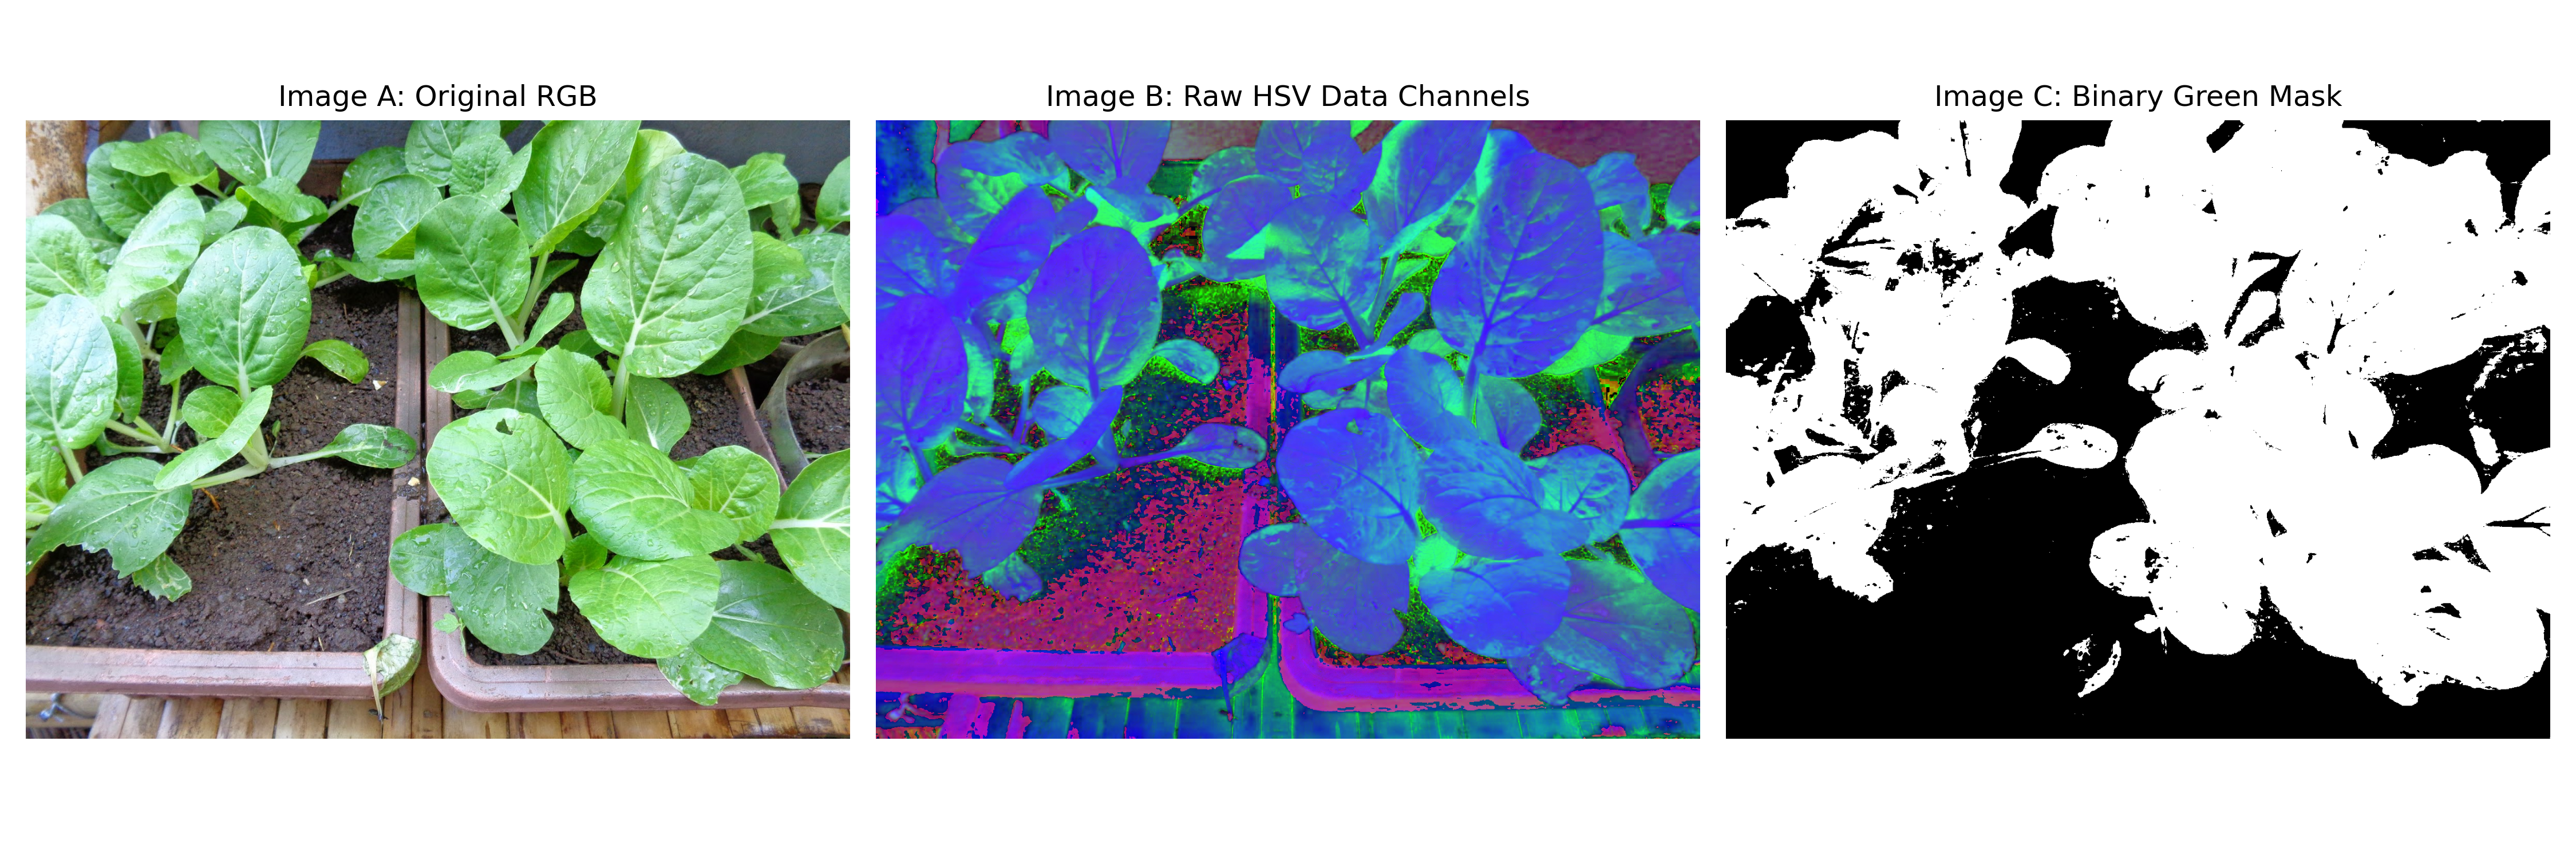
\includegraphics[width=\linewidth]{RGB_vs_HSV_Filtering_1.png}
    \caption{Visual comparison of RGB image capture, HSV color-space conversion, and binary vegetation masking for green canopy segmentation.}
    \label{fig:rgb-hsv-filtering}
\end{figure}

%section 2.3
\section{Resource-Constrained Edge Computing for Agricultural Vision}

Early architectural frameworks for agricultural image processing relied heavily on continuous cloud-computing pipelines. In these traditional setups, localized microcontrollers functioned merely as raw telemetry nodes, capturing image payloads and transmitting them to remote servers (e.g., Firebase or AWS) where high-level segmentation algorithms were executed. While cloud architectures offer virtually unlimited computational scalability, they introduce severe operational vulnerabilities in residential or provincial deployments. Continuously streaming high-resolution image data consumes massive internet bandwidth and makes the system entirely dependent on external network stability. A localized Wi-Fi outage results in complete data loss for that day, corrupting the time-series continuity required for accurate yield modeling.

To resolve these latency and dependency vulnerabilities, modern IoT frameworks have shifted the computational burden to the localized point of data collection—a paradigm known in the literature as Edge Computing \cite{Shi2016}. Single Board Computers (SBCs), such as the Raspberry Pi Zero 2W, offer an optimal hardware platform for agricultural edge inference. Unlike basic microcontrollers, SBCs provide a full Linux-based operating system, dedicated RAM, and enough localized processing capability to natively execute computer vision scripts (such as OpenCV-based HSV thresholding) \cite{Zamora2019}. By processing the image locally at the edge, the system extracts the vital numerical data (the Green Pixel Ratio) and discards the heavy image file. This ensures that the system operates completely autonomously and offline, storing daily numerical metrics directly into local CSV files on the edge device without requiring internet connectivity or external server infrastructure.

While Single Board Computers provide necessary processing power for computer vision, they present a significant power-management challenge. SBCs fundamentally lack the microampere deep-sleep architectures native to standard microcontrollers. Consequently, running a Raspberry Pi continuously in a 24-hour cycle introduces an idle-current drain that, while manageable in laboratory settings, requires careful thermal management in greenhouse environments.

The present study adopts this localized processing philosophy, but implements it through an always-on architecture for the Raspberry Pi Zero 2W. This approach eliminates boot-cycle hardware failures and filesystem corruption risks associated with repeated hard power-cycling, ensuring reliable daily image capture. The ESP32-S3, operating on a separate low-power rail, manages sensor polling and irrigation actuation independently. This cooperative architecture ensures the system achieves the complex analytical capabilities of a full computer vision setup while maintaining reliable long-term operation in a greenhouse environment.

%section 2.4
\section{Crop Yield Prediction and Predictive Modeling Mechanics}

The final analytical objective of an agricultural computer vision pipeline is the translation of localized structural data, specifically the daily Green Pixel Ratio (GPR), into an accurate estimation of final harvest biomass. In contemporary precision agriculture, Deep Learning (DL) architectures, such as Convolutional Neural Networks (CNNs) and Long Short-Term Memory (LSTM) networks, are frequently deployed for yield forecasting. While these models exhibit exceptional predictive capabilities in large-scale commercial deployments, literature clearly identifies their fundamental limitations when applied to short-term, resource-constrained academic environments \cite{Kamilaris2018}. 

Deep learning networks inherently act as "black box" algorithms that require massive datasets, often spanning thousands of annotated images collected across multiple historical grow-out seasons, to establish valid statistical weights. Attempting to train a deep neural network on a single-semester cultivation cycle with a limited localized crop sample invariably results in catastrophic overfitting. In such scenarios, the model merely memorizes the specific training data anomalies rather than learning generalizable biological growth patterns. Consequently, for localized, rapid-deployment IoT frameworks, empirical statistical modeling provides a substantially more robust and mathematically transparent alternative. By utilizing defined mathematical regression equations, statistical models map the time-series GPR data directly to ground-truth fresh-weight measurements without requiring the vast, multi-season datasets necessary for neural network convergence.

To achieve high predictive accuracy via statistical modeling, the mathematical architecture of the regression curve must mirror the natural physiological growth patterns of the target crop. While simple Linear Regression models are computationally straightforward, they assume a continuous, straight-line relationship between time and biomass accumulation. Agronomic literature establishes that biological plant development does not scale linearly without limit; rather, crops follow a curvilinear or sigmoidal progression. Plants exhibit rapid exponential vegetative expansion during their early and middle life stages, followed by a distinct physiological deceleration or plateau as they reach reproductive maturity or harvest readiness \cite{Ge2016}.

Applying a linear equation to this biological reality frequently results in severe predictive errors during the late-stage growth plateau, as illustrated in Fig.~\ref{fig:regression-comparison}. Therefore, nonlinear mathematical frameworks, specifically second-degree (\(2^{nd}\)) or third-degree (\(3^{rd}\)) Polynomial Regression models, are widely validated as the optimal approach for non-destructive plant phenotyping \cite{Archontoulis2015}. A polynomial curve mathematically accounts for the natural deceleration of vegetative canopy spread, allowing the model to calculate a highly accurate line of best fit that correlates a specific temporal data point (e.g., the cumulative GPR extracted on Day 20) with the final fresh-weight biomass measured in grams at harvest. 

The integrity and predictive performance of these empirical models are evaluated using universally standardized statistical metrics. The coefficient of determination (\(R^2\)) is utilized to quantify the proportion of biological variance accurately explained by the polynomial curve, with values approaching 1.0 indicating a mathematically stable relationship. Concurrently, the Mean Absolute Error (MAE) is employed to measure the average magnitude of absolute prediction discrepancies between the calculated yield and the physical ground-truth scale weight. Utilizing these specific mathematical dynamics ensures that the yield prediction pipeline remains academically rigorous, highly transparent, and computationally efficient at the edge.

\begin{figure}[htbp]
    \centering
    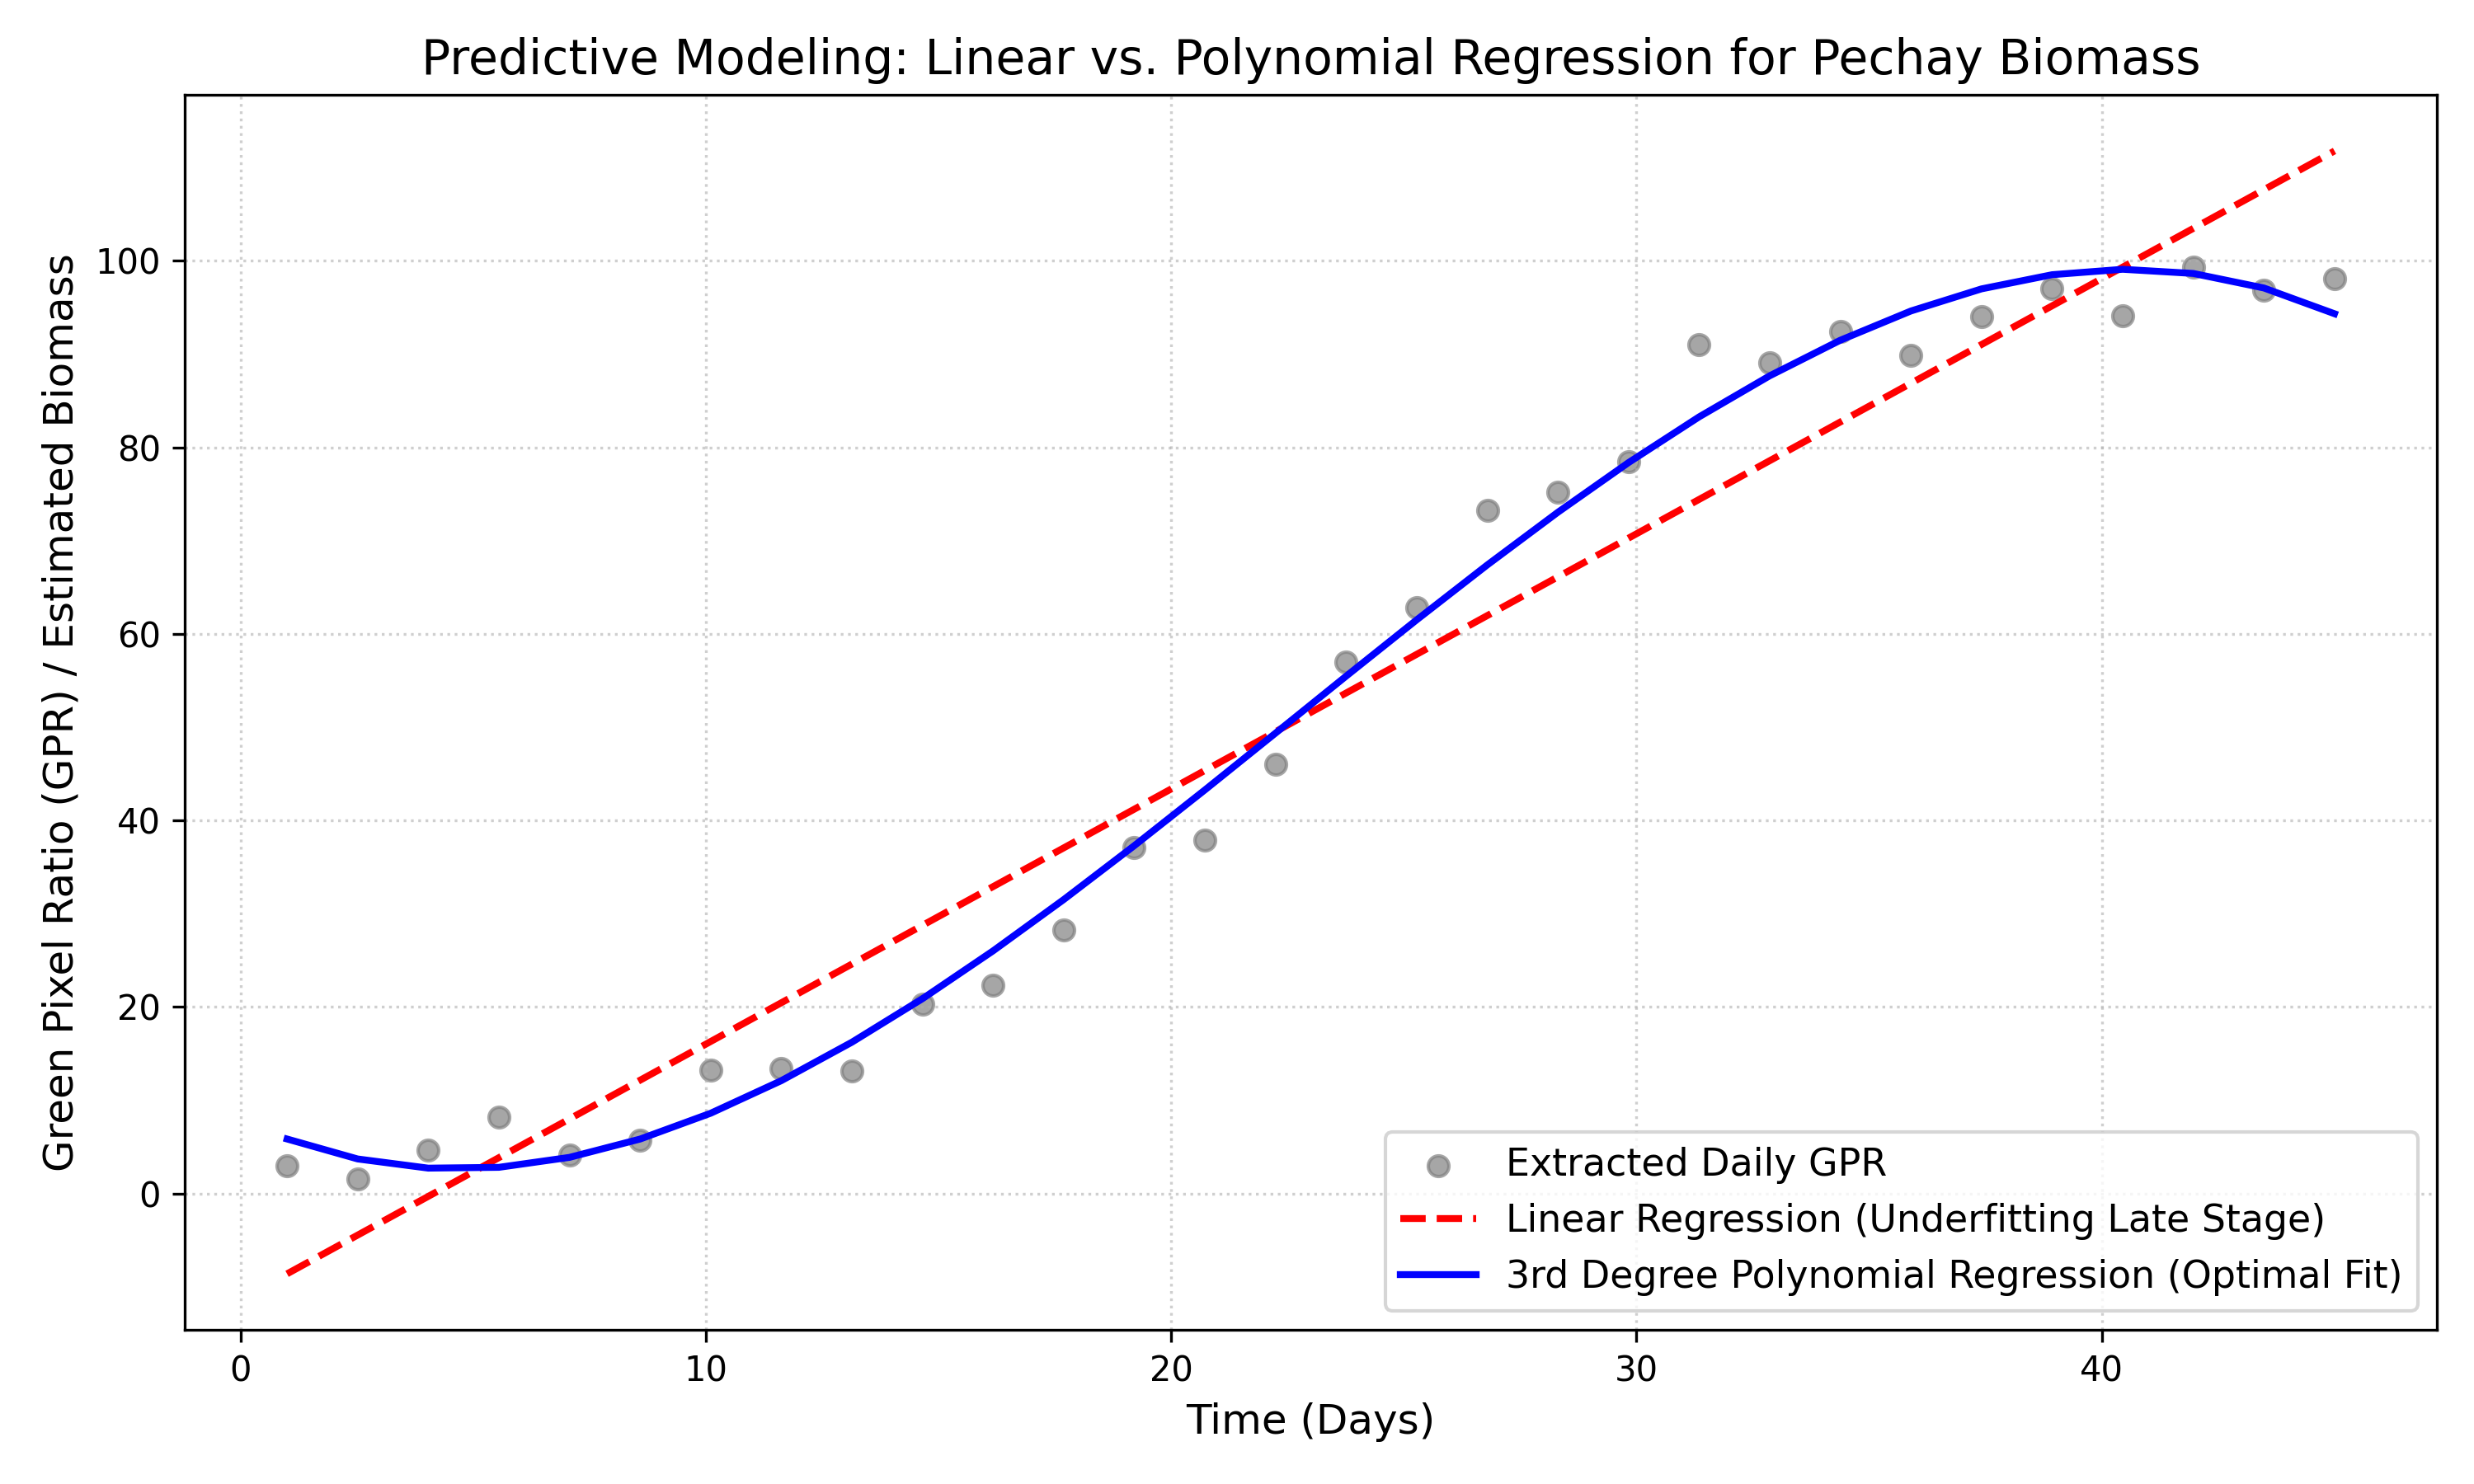
\includegraphics[width=\linewidth]{Regression_Comparison.png}
    \caption{Comparison of linear and polynomial regression fits for nonlinear plant growth progression over time.}
    \label{fig:regression-comparison}
\end{figure}

\FloatBarrier

%section 2.5
\section{Agronomic Variable Controls in Modeling Environments}

A predictive mathematical regression model is fundamentally reliant on the integrity and consistency of its input parameters. In vision-based phenotyping, if the daily Green Pixel Ratio (GPR) fluctuates erratically, the resulting statistical curve will fail, yielding a low \(R^2\) score and a high Mean Absolute Error (MAE). Agronomic literature establishes that in unregulated or open-field agricultural setups, visual data is heavily corrupted by uncontrollable environmental noise. Fluctuating outdoor sunlight intensities, passing cloud cover, and dynamic shadow casting severely alter the perceived color vectors of a plant canopy, causing vision algorithms to misclassify shadow pixels as background soil \cite{Slaughter2008}. Furthermore, wind-induced mechanical stress can temporarily alter the orientation of the leaves during image capture, introducing false drops in the recorded GPR.

To secure the mathematical stability of the predictive model, strict agronomic control variables must be enforced through physical environmental isolation. Cultivating target crops within a controlled greenhouse setting natively mitigates weather anomalies and wind disturbances. More critically, a greenhouse environment allows for the implementation of standardized, enclosed LED lighting structures. By triggering the camera module only during periods of controlled, uniform artificial illumination, the system actively neutralizes dynamic shadow masks and ambient light shifts. This physical standardization guarantees that daily GPR extractions are uniform, ensuring that the regression model maps true biological progression rather than random environmental artifacts.

Beyond visual noise, the physical cultivation architecture directly impacts the physiological validity of the yield prediction model. Early iterations of residential agriculture frequently utilize shared, open crop plots where multiple seedlings are cultivated within a single, continuous soil volume. However, plant physiological studies consistently demonstrate that in shared root zones, crops compete asymmetrically for available water, physical space, and localized macronutrients \cite{Poorter2012}. In such environments, a faster-growing specimen will naturally extend its root network, depriving adjacent plants of moisture. This hidden root-zone competition introduces severe localized stress vectors. As a result, two plants exhibiting identical visual canopy sizes (equal GPR) might possess vastly different physical harvest weights due to unequal nutrient accumulation, which completely invalidates the mathematical correlation required for a statistical yield model.

To eliminate this biological variance, literature strongly advocates for data isolation through the use of individual, uniform cultivation containers. Cultivating each specimen in an isolated pot utilizing standardized soil media strictly bounds the rooting volume and neutralizes inter-plant competition \cite{Poorter2012}. Furthermore, coupling individual pot isolation with an automated 1:1 irrigation baseline ensures that every single plant maintains an identical, optimal soil moisture capacity. By removing watering anomalies and nutrient competition from the equation, the experimental environment is thoroughly sanitized. Consequently, any quantifiable change in the daily Green Pixel Ratio is purely and exclusively a reflection of unpolluted biological growth, providing the pristine data points required to train a highly defensible and accurate statistical regression model.

%section 2.6
\section{Prior Institutional Studies as the Validated Baseline Framework}

The experimental framework of the present study is grounded in a direct lineage of institutional research conducted at the University of San Carlos. Aala et al. (2022) established the foundational proof-of-concept for IoT-based automated urban farming, deploying capacitive soil moisture sensors and a modular sprinkler probe system in a shared soil plot \cite{Aala2022}. Their system demonstrated basic automated irrigation capability but encountered critical sensor reliability issues, specifically, the continuous immersion of a glass-bulb pH probe in soil caused progressive signal drift requiring frequent manual recalibration, and loose jumper wire interconnects in the humid growing environment introduced intermittent data faults \cite{Aala2022}. Critically, no plant health monitoring of any kind was automated in their system; the researchers acknowledged this as an open direction for future work, suggesting further studies with actual crop planting and monitoring be conducted \cite{Aala2022}.

Zamora et al. (2025) built directly on this foundation, replacing the unstable pH probe dependency with a simplified architecture focused on capacitive soil moisture sensors and solenoid-actuated irrigation probes embedded in a shared \(0.4\,\mathrm{m} \times 1.0\,\mathrm{m}\) crop plot \cite{ZamoraOgue2025}. Their comparative grow-out trial demonstrated that automated moisture-threshold irrigation produced Pechay with a 92.1\% higher average fresh weight than manual watering, validating the effectiveness of sensor-driven automation for urban crop cultivation \cite{ZamoraOgue2025}. However, plant health assessment throughout the entire 37-day grow-out period was conducted exclusively through daily manual measurements, as a researcher physically measured each plant's height with a ruler, counted its leaves, and assessed leaf color using a standardized IRRI Leaf Color Chart \cite{ZamoraOgue2025}. No automated visual monitoring existed at any point during data collection. This labor-intensive manual process confirmed that while the irrigation layer had been solved and validated, the plant monitoring layer remained entirely unaddressed across both institutional iterations.

By inheriting and redeploying the validated automated irrigation approach from Zamora et al. (2025) while transitioning from a shared crop plot to individual isolated container pots, the present study eliminates the need to re-establish irrigation hardware credibility and directs its original contribution entirely toward the computer vision and statistical modeling pipeline, the layer that both prior iterations identified as absent but did not address.
